\documentclass[tikz]{standalone}
\usetikzlibrary{calc}

\begin{document}

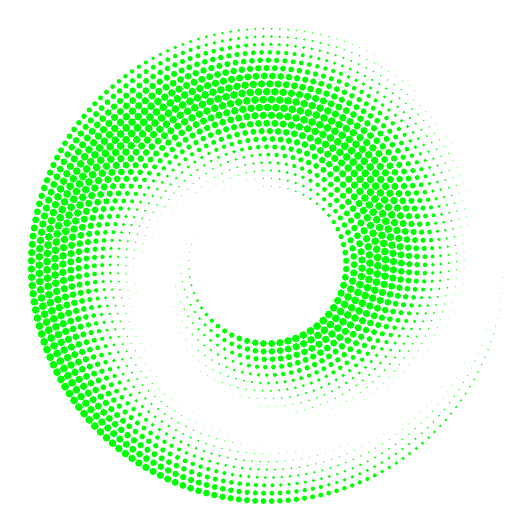
\begin{tikzpicture}

\pgfmathsetmacro\maxradius{.5}

\foreach \stepy in {10, ..., 30}
    \pgfmathsetmacro\stepstart{60/\stepy}
    \pgfmathsetmacro\steplast{360-\stepstart}
    \pgfmathsetmacro\stepcount{floor(360/\stepstart)}
    \foreach \stepx in {0, \stepstart, ..., \steplast}
        \pgfmathsetmacro\stepsingle{floor(\stepx/\stepstart)}
        \pgfmathsetmacro\stepradius{(\maxradius/2)*cos(deg(\stepsingle*pi/(\stepcount/2) - pi - (\stepy/5))) + (\maxradius/2)}
        \fill[green] ({\stepx+.25*\stepcount}:\stepy mm) circle (\stepradius mm);

\end{tikzpicture}

\end{document}

